% Options for packages loaded elsewhere
\PassOptionsToPackage{unicode}{hyperref}
\PassOptionsToPackage{hyphens}{url}
\PassOptionsToPackage{dvipsnames,svgnames,x11names}{xcolor}
\documentclass[
  british,
  11pt,
  a4paper,
]{article}
\usepackage{xcolor}
\usepackage[margin=25mm]{geometry}
\usepackage{amsmath,amssymb}
\setcounter{secnumdepth}{5}
\usepackage{iftex}
\ifPDFTeX
  \usepackage[T1]{fontenc}
  \usepackage[utf8]{inputenc}
  \usepackage{textcomp} % provide euro and other symbols
\else % if luatex or xetex
  \usepackage{unicode-math} % this also loads fontspec
  \defaultfontfeatures{Scale=MatchLowercase}
  \defaultfontfeatures[\rmfamily]{Ligatures=TeX,Scale=1}
\fi
\usepackage{lmodern}
\ifPDFTeX\else
  % xetex/luatex font selection
\fi
% Use upquote if available, for straight quotes in verbatim environments
\IfFileExists{upquote.sty}{\usepackage{upquote}}{}
\IfFileExists{microtype.sty}{% use microtype if available
  \usepackage[]{microtype}
  \UseMicrotypeSet[protrusion]{basicmath} % disable protrusion for tt fonts
}{}
\makeatletter
\@ifundefined{KOMAClassName}{% if non-KOMA class
  \IfFileExists{parskip.sty}{%
    \usepackage{parskip}
  }{% else
    \setlength{\parindent}{0pt}
    \setlength{\parskip}{6pt plus 2pt minus 1pt}}
}{% if KOMA class
  \KOMAoptions{parskip=half}}
\makeatother
\usepackage{longtable,booktabs,array}
\newcounter{none} % for unnumbered tables
\usepackage{calc} % for calculating minipage widths
% Correct order of tables after \paragraph or \subparagraph
\usepackage{etoolbox}
\makeatletter
\patchcmd\longtable{\par}{\if@noskipsec\mbox{}\fi\par}{}{}
\makeatother
% Allow footnotes in longtable head/foot
\IfFileExists{footnotehyper.sty}{\usepackage{footnotehyper}}{\usepackage{footnote}}
\makesavenoteenv{longtable}
\usepackage{graphicx}
\makeatletter
\newsavebox\pandoc@box
\newcommand*\pandocbounded[1]{% scales image to fit in text height/width
  \sbox\pandoc@box{#1}%
  \Gscale@div\@tempa{\textheight}{\dimexpr\ht\pandoc@box+\dp\pandoc@box\relax}%
  \Gscale@div\@tempb{\linewidth}{\wd\pandoc@box}%
  \ifdim\@tempb\p@<\@tempa\p@\let\@tempa\@tempb\fi% select the smaller of both
  \ifdim\@tempa\p@<\p@\scalebox{\@tempa}{\usebox\pandoc@box}%
  \else\usebox{\pandoc@box}%
  \fi%
}
% Set default figure placement to htbp
\def\fps@figure{htbp}
\makeatother
\ifLuaTeX
\usepackage[bidi=basic,shorthands=off]{babel}
\else
\usepackage[bidi=default,shorthands=off]{babel}
\fi
\ifLuaTeX
  \usepackage{selnolig} % disable illegal ligatures
\fi
\setlength{\emergencystretch}{3em} % prevent overfull lines
\providecommand{\tightlist}{%
  \setlength{\itemsep}{0pt}\setlength{\parskip}{0pt}}
\usepackage{needspace}
\usepackage{bookmark}
\IfFileExists{xurl.sty}{\usepackage{xurl}}{} % add URL line breaks if available
\urlstyle{same}
\hypersetup{
  pdftitle={Integer calendars for fixed-turnover replenishment},
  pdfauthor={Anonymous},
  pdflang={en-GB},
  colorlinks=true,
  linkcolor={violet},
  filecolor={Maroon},
  citecolor={Blue},
  urlcolor={teal},
  pdfcreator={LaTeX via pandoc}}

\title{Integer calendars for fixed-turnover replenishment}
\usepackage{etoolbox}
\makeatletter
\providecommand{\subtitle}[1]{% add subtitle to \maketitle
  \apptocmd{\@title}{\par {\large #1 \par}}{}{}
}
\makeatother
\subtitle{A 1/ln 2 guarantee on trees, the price of short cycles and the
price of constant gaps}
\author{Anonymous}
\date{31 October 2026 · Release 1.0.0-candidate · DOI
10.5281/zenodo.23845965}

\begin{document}
\maketitle

{
\setcounter{tocdepth}{2}
\tableofcontents
}
\section*{Abstract}\label{abstract}
\addcontentsline{toc}{section}{Abstract}

A depot must revisit every client at least once within that client's own
number of days, its \emph{turnover time}, while keeping the long-run
average daily routing cost low. Bosman et al.~(2022) gave a factor-two
approximation on tree networks and asked whether it could be improved.
It can. We give every client a real-valued clock from one shared ladder
of periods, choose the ladder's offset by a logarithmic averaging
argument, and round each clock's event times up to whole days. The
resulting calendar meets every deadline and costs at most
\(1/\ln2\approx1.4427\) times the optimum. It is computed
deterministically in \(O(n\log n)\) time, for any monotone submodular
daily cost, of which tree routing is one case. The calendar repeats
within the longest turnover time, and for such calendars \(1/\ln2\) is
the exact worst-case price. A client's gaps may alternate between two
consecutive integers. If every client must instead keep a constant gap,
with the gaps dividing one another (the form of Bosman et al.'s output),
the best possible worst-case factor lies between \(1.6001\) and
\(1.6014\). We also solve the nested two-edge problem exactly,
characterise when the standard frequency lower bound is attained, and
certify optimal schedules for small trees in exact arithmetic. The
rounding tools and the constant are classical. Our contribution is their
integer-calendar realisation and the structural bounds. A 2025 master's
thesis with a closely matching title could not be obtained, so we do not
claim priority.

\textbf{Keywords:} inventory routing; fixed turnover times; recurring
service; submodular costs; approximation algorithms; harmonic schedules;
pinwheel scheduling.

\section{Introduction}\label{introduction}

\subsection{The problem in plain
terms}\label{the-problem-in-plain-terms}

Picture a depot that restocks cash machines, fuel tanks or vending
machines spread along a branching road network. Client \(i\) holds
enough stock for \(\tau_i\) days, its turnover time, so it must be
visited at least once in every window of \(\tau_i\) consecutive days.
Each day a vehicle leaves the depot, visits that day's clients and
returns. On a tree network, a day's cost is the length of road it uses,
travelled out and back. A visit to one client makes the road to its
neighbours already partly paid for. Planners therefore want to
\emph{synchronise} visits so that clients sharing a road are served on
the same days.

Synchronisation has a catch. Visiting a client early, to share a trip,
resets its clock, and its next deadline then arrives earlier too.
Knowing how often each client should be visited on average is not
enough. Every rolling deadline must hold on every day. The question is
how cheaply a feasible calendar can be built, and how close to the best
possible long-run average cost it can come.

Bosman et al.~(2022) introduced this \emph{replenishment problem with
fixed turnover times} (first presented at LATIN 2018). For trees, they
rounded every turnover time down to a power of two and visited each
client on the multiples of its rounded period. This gives a feasible
calendar whose average cost is at most twice the optimum. They asked
whether the factor two could be improved (their Section 5). The same
question is restated in Bosman's thesis (2019, Chapter 3).

\subsection{What this paper shows}\label{what-this-paper-shows}

Table 1 summarises the results. Section 2 sets up the model, and
Sections 3--4 prove the main guarantee and apply it to trees. Section 5
gives exact structural bounds, Section 6 the limits of short cycles,
Section 7 the constant-gap results, Section 8 the computations and
Section 9 the practical reading and the limitations.

\Needspace{12\baselineskip}

\begin{longtable}[]{@{}
  >{\raggedright\arraybackslash}p{(\linewidth - 6\tabcolsep) * \real{0.2727}}
  >{\raggedright\arraybackslash}p{(\linewidth - 6\tabcolsep) * \real{0.1273}}
  >{\raggedright\arraybackslash}p{(\linewidth - 6\tabcolsep) * \real{0.3273}}
  >{\raggedright\arraybackslash}p{(\linewidth - 6\tabcolsep) * \real{0.2727}}@{}}
\caption{Results at a glance. ``Tight'' refers to worst-case ratios
against the unrestricted optimum.}\tabularnewline
\toprule\noalign{}
\begin{minipage}[b]{\linewidth}\raggedright
Setting
\end{minipage} & \begin{minipage}[b]{\linewidth}\raggedright
Previously known
\end{minipage} & \begin{minipage}[b]{\linewidth}\raggedright
This paper
\end{minipage} & \begin{minipage}[b]{\linewidth}\raggedright
Tight?
\end{minipage} \\
\midrule\noalign{}
\endfirsthead
\toprule\noalign{}
\begin{minipage}[b]{\linewidth}\raggedright
Setting
\end{minipage} & \begin{minipage}[b]{\linewidth}\raggedright
Previously known
\end{minipage} & \begin{minipage}[b]{\linewidth}\raggedright
This paper
\end{minipage} & \begin{minipage}[b]{\linewidth}\raggedright
Tight?
\end{minipage} \\
\midrule\noalign{}
\endhead
\bottomrule\noalign{}
\endlastfoot
Trees, average cost (calendars may vary individual gaps) & factor 2
(Bosman et al.) & \(1/\ln2\approx1.4427\) (Theorem 1, Corollary 1) & Yes
for the algorithm and for every calendar repeating within
\(\tau_{\max}\) (Theorem 7, Corollary 2) \\
Monotone submodular daily cost & --- & \(1/\ln2\) (Theorem 1) & Same \\
Constant gaps that divide one another (form of Bosman et al.'s output) &
factor 2 & between \(1.6001\) and \(1.6014\); \(48/29\) with four
ladders (Theorem 9) & Bracket of width \(0.0013\) \\
Two nested edges & --- & exact optimum (Theorem 2) & Exact \\
When the frequency lower bound is attained & --- & divisibility and lcm
criteria (Theorems 3, 5) & Exact \\
Cost of a longer global cycle on the witness family & --- & full
limiting profile (Theorem 8) & Exact asymptotics \\
\end{longtable}

The main idea fits in one sentence. Classical inventory theory picks
real-valued periods from a common power-of-two ladder with a well-chosen
offset. We keep those real periods and round each \emph{event time}
\(k p_i\) up to an integer day, rather than rounding the \emph{periods}.
Rounding event times keeps every gap at most
\(\lceil p_i\rceil\le\tau_i\) and keeps clients that share a road
synchronised. Rounding periods to integers would break one property or
the other. Because of this, a client with period \(3/2\) is served with
gaps \(2,1,2,1,\ldots\): its gaps are not constant, but it is never
late.

That last feature is the honest boundary of the main result. Bosman et
al.~defined feasibility through rolling windows, and their optimum
ranges over all repeating schedules. For compact output, though, they
chose to consider only \emph{periodic} solutions, in which each client
keeps a constant gap (their Section 1). Our \(1/\ln2\) guarantee
compares against the same optimum as theirs, but the calendars it
produces lie outside that output class. Section 7 therefore asks what is
possible inside it. Constant gaps that divide one another can also beat
two, but they cannot approach \(1/\ln2\): the best factor is about
\(1.60\).

\subsection{Related work and credit}\label{related-work-and-credit}

\emph{Classical rounding.} Power-of-two policies originate with Roundy
(1985). Roundy (1989) showed that feasibility-preserving rounding to
powers of two loses at most about 44\% in capacitated lot sizing, which
is the factor \(1/\ln2\). Federgruen and Zheng (1992) treat joint
replenishment with monotone submodular setup costs. Federgruen and Zheng
(1993) optimise fixed-base power-of-two policies with upper and lower
bounds on reorder intervals. Teo and Bertsimas (2001, Sections 2.3 and
3) use logarithmic random shifts and the greedy representation of
submodular costs. Their resource-constrained algorithm rounds periods
\emph{up} to respect frequency bounds, which is the wrong direction for
maximum-gap constraints. Segev (2026) reports \(5/(6\ln2)\) for
continuous resource-constrained joint replenishment, using upward-closed
interval constraints that do not include hard maximum gaps. Cheung et
al.~(2016) and Nagarajan and Shi (2016) study joint replenishment with
submodular or routing costs over a finite horizon with given demands.
Zhang and Kulkarni (2018) study a stochastic automated-teller-machine
model with submodular costs; we inspected only its abstract. We use all
these ingredients and credit them as such.

\emph{Deadline aggregation.} Over a finite horizon, each rolling
constraint ``serve \(i\) in \([t+1,t+\tau_i]\)'' is a request with a
release time and a deadline. The tree problem then becomes multilevel
aggregation with deadlines. Becchetti et al.~(2009) and Bienkowski et
al.~(2020) give factor-two offline algorithms for that problem. On a
depth-two tree it is the joint replenishment problem with deadlines, for
which Bienkowski et al.~(2015) give a \(1.574\)-approximation, LP
integrality-gap lower bounds and APX-hardness (Nonner and Souza, 2009,
gave \(5/3\)). These routes need the horizon, and hence the \(\tau_i\),
to be written out day by day. They are therefore pseudo-polynomial in
the compact input, and they have boundary effects at the ends of the
horizon. Theorem 1 improves on every factor available through them, in
polynomial time. Their hardness results are for general windows and do
not obviously transfer to rolling periodic windows. Bosman et
al.~conjecture that the tree problem is hard, but its complexity remains
open.

\emph{Pinwheel and real-time scheduling.} Constraint (1) below is the
defining constraint of pinwheel scheduling (Holte et al., 1989), where
at most one client may be served per day and the question is
feasibility. In its single-integer reduction, Chan and Chin specialise
periods to one ladder of the form \(x\,2^k\) (Chan and Chin, 1992,
1993). The asymptotic density threshold \(\ln2\) of that reduction is
the feasibility counterpart of our Theorem 6. Kawamura (2024) proved the
\(5/6\) density conjecture. Fujiwara, Miyagi and Ouchi (2026) study a
real-period pinwheel variant attributed to Kawamura, in which a task of
real period \(a\) must be served at least \(l\) times in every
\(\lceil la\rceil\) consecutive days. Our rounded clocks (7) satisfy
exactly this property, so the rounding of real periods to integer days
has close precedent there. Our setting differs in having no daily
capacity and a cost objective. The \(\ln2\) in the rate-monotonic
utilisation bound of Liu and Layland (1973) has the same octave origin.
Han and Lin (1992) and Han, Lin and Hou (1996) specialise real periods
to a base times powers of two for distance-constrained tasks, which have
integer slots and maximum gaps. We could not inspect those full texts,
so they may contain an equivalent integer-slot realisation. The harmonic
specialisation attributed to Han and Tyan is reproduced as Algorithm 2
of Díaz-Ramírez et al.~(2013). Identifying task periods with turnovers
and execution costs with the weights \(a_i\), its \(O(n\log n)\)
breakpoint optimisation coincides with our clock-selection step. We do
not claim that sweep as new. Mohaqeqi et al.~(2018) and Bhat and
Rajkumar (2023) study real and integer harmonic period assignment under
upper bounds. Bamboo-garden trimming (van Ee, 2021) and perpetual
maintenance (Gąsieniec et al., 2024) are further relatives of the
problem, as are periodic maintenance and cost-minimising periodic
service (Anily, Glass and Hassin, 1998; Bar-Noy et al., 2002). Coelho,
Cordeau and Laporte (2014) survey inventory routing.

\emph{The problem's own history.} Bosman et al.~also give an
\(O(\log n)\) algorithm for general metrics. Bosman and Olver (2020) and
Bosman (2019) improve this to \(O(\log\log n)\). Corollary 1 combined
with tree embeddings does not improve the general-metric bound. Bosman's
thesis is open access. We read its Chapter 3: it contains the factor two
for trees and the same open question, and no logarithmic shift. A
university supervision page also lists Hans Henrik Hermansen's Spring
2025 MSc thesis, \emph{Approximation Algorithms for Replenishment
Problems with Fixed Turnover Times} (Technical University of Denmark).
We could not obtain its text. It has no Crossref, arXiv or Semantic
Scholar record, its supervision page links no file, and the university
catalogues were not accessible to automated search. Its contents are
therefore unknown, and it could contain an equivalent or stronger
result. The bundled novelty report records every query and source
boundary.

\section{Model}\label{model}

Let \(N=\{1,\ldots,n\}\) be the clients. Each client \(i\) has a
positive integer turnover time \(\tau_i\). On day \(t\ge1\), a schedule
serves a set \(S_t\subseteq N\). Feasibility means

\[
i\in\bigcup_{s=t+1}^{t+\tau_i}S_s
\qquad\text{for every }i\in N\text{ and every integer }t\ge0. \tag{1}
\]

For a schedule that repeats with cycle \(P\) (a \emph{\(P\)-periodic}
schedule, \(S_{t+P}=S_t\)), condition (1) also applies across the cycle
boundary. Equivalently, every gap between successive services of client
\(i\) is at most \(\tau_i\).

The daily cost is a set function \(f:2^N\to\mathbb R_{\ge0}\) with
\(f(\varnothing)=0\). We assume that it is monotone and has diminishing
returns:

\[
f(A)\le f(B)\quad(A\subseteq B),
\]

\[
f(A\cup\{i\})-f(A)\ge f(B\cup\{i\})-f(B)
\quad(A\subseteq B,\ i\notin B). \tag{2}
\]

The second condition is submodularity. In the tree example, it says that
a client whose road is already on today's route costs at most the extra
branch to reach it. It is an assumption about the given cost function;
the algorithm does not test it.

For a \(P\)-periodic calendar, the objective is

\[
\overline C=\frac1P\sum_{t=1}^P f(S_t).
\]

Let \(\operatorname{OPT}\) be the infimum over feasible repeating
calendars, with no constant-gap restriction for individual clients. The
lower bounds below also apply to arbitrary feasible schedules through
limiting averages. For rational inputs and a rational value oracle, all
arithmetic in the construction is exact.

Relabel the clients so that \(\tau_1\le\cdots\le\tau_n\). Define
\(N_i=\{1,\ldots,i\}\), \(N_0=\varnothing\), and

\[
a_i=f(N_i)-f(N_{i-1}),\qquad
L_f=\sum_{i=1}^n\frac{a_i}{\tau_i},\qquad
W_1=\sum_{i:\tau_i=1}a_i. \tag{3}
\]

Ties can be ordered arbitrarily; the expressions are unchanged after
summing within groups of equal turnover. Monotonicity gives \(a_i\ge0\).

\emph{Terminology.} A \textbf{clock} is a real period \(p_i\) with
events at \(p_i,2p_i,\ldots\). A \textbf{calendar} is the resulting
integer-day service pattern. A family of periods is \textbf{harmonic}
(in the scheduling sense, not the harmonic numbers \(H_k\) that also
appear below) if each larger period is an integer multiple of each
smaller one. A \textbf{ladder} is such a family, and its \textbf{phase}
fixes its position on the logarithmic scale.

\textbf{Theorem 1 (integer-calendar approximation).} There is a
deterministic algorithm, using \(n+1\) value-oracle calls and
\(O(n\log n)\) arithmetic operations, that returns a feasible repeating
calendar satisfying

\[
\overline C\le W_1+\frac{L_f-W_1}{\ln2}
\le\frac{L_f}{\ln2}
\le\frac{\operatorname{OPT}}{\ln2}. \tag{4}
\]

The calendar has an integer cycle \(P\le\tau_{\max}=\max_i\tau_i\).
Apart from the costs and client labels, it is described by
\(O(n\log(1+\tau_{\max}))\) bits, and any day's service set can be
generated without expanding the cycle.

The operation count does not assume that rational arithmetic has unit
bit cost. With polynomially encoded rational oracle answers, every
intermediate numerator and denominator has polynomial bit length, so the
algorithm is polynomial in the standard bit model too. If
\(\operatorname{OPT}=0\) (for example \(f\equiv0\)), then \(L_f=0\),
every \(a_i=0\), and the calendar costs zero, so (4) holds trivially.

\section{Proof of the calendar
theorem}\label{proof-of-the-calendar-theorem}

\subsection{A lower bound from
submodularity}\label{a-lower-bound-from-submodularity}

\textbf{Lemma 1 (greedy supporting weights).} For every
\(S\subseteq N\),

\[
f(S)\ge\sum_{i\in S}a_i. \tag{5}
\]

\textbf{Proof.} Insert the elements of \(S\) in increasing index order.
Immediately before \(i\) is inserted, the inserted set is contained in
\(N_{i-1}\). Diminishing returns implies that the marginal cost of
inserting \(i\) is at least \(f(N_i)-f(N_{i-1})=a_i\). Summing these
marginal inequalities proves (5). \(\square\)

Over a cycle, client \(i\) must be served on at least a fraction
\(1/\tau_i\) of the days, because its gaps average at most \(\tau_i\).
Applying (5) on each day and averaging proves
\(\operatorname{OPT}\ge L_f\), since the weights \(a_i\) are
nonnegative. For a noncyclic horizon of \(T\) days, disjoint blocks
force at least \(\lfloor T/\tau_i\rfloor\) visits, and the same bound
follows after dividing by \(T\) and letting \(T\to\infty\). The quantity
\(L_f\) is the Lovász extension of \(f\) at the frequency vector
\((1/\tau_i)_i\), but the elementary proof suffices here. We call
\(L_f\) the \textbf{frequency bound}.

\subsection{Harmonic clocks and integer
days}\label{harmonic-clocks-and-integer-days}

For \(1\le\alpha<2\), define

\[
p_i(\alpha)=\alpha\,2^{\lfloor\log_2(\tau_i/\alpha)\rfloor}. \tag{6}
\]

Thus \(p_i\le\tau_i<2p_i\). Serve client \(i\) on the distinct days in

\[
D_i(\alpha)=\{\lceil k p_i(\alpha)\rceil:k=1,2,\ldots\}. \tag{7}
\]

Internal events that land on the same day generate one service, not
several charges.

\textbf{Lemma 2 (feasibility, nesting and frequency).} The calendars (7)
satisfy (1). If \(i<j\), then \(D_j\subseteq D_i\). The limiting
fraction of days in \(D_i\) is

\[
\rho_i(\alpha)=\min\{1,1/p_i(\alpha)\}. \tag{8}
\]

\textbf{Proof.} If \(p_i\ge1\), successive rounded events have gaps of
\(\lfloor p_i\rfloor\) or \(\lceil p_i\rceil\le\tau_i\), and the first
event falls no later than day \(\lceil p_i\rceil\le\tau_i\). Once the
calendar is shown to repeat with cycle \(P\), where \(P\) is a multiple
of \(p_i\) (Section 3.5), the gap across the cycle boundary is the gap
from day \(P\) to day \(P+\lceil p_i\rceil\), which also equals
\(\lceil p_i\rceil\). If \(p_i<1\), the integer sequence
\(\lceil k p_i\rceil\) increases by zero or one and eventually reaches
every positive integer, so the client is served daily. This covers the
subday clocks that arise for \(\tau_i=1\).

Because \(\tau_i\le\tau_j\), the ratio \(p_j/p_i\) is a nonnegative
integer power of two. Every event \(k p_j\) is therefore also an event
of the shorter clock before rounding, and rounding both in the same way
preserves the inclusion of their event days.

For \(p_i\ge1\), no events coalesce, and the number of events up to day
\(T\) is \(\lfloor T/p_i\rfloor\), so the density is \(1/p_i\). For
\(p_i<1\), every day is active and the density is one. \(\square\)

Every daily service set is therefore a prefix \(N_i\), possibly empty.
Its cost telescopes exactly as \(f(S_t)=\sum_{i\in S_t}a_i\), and the
limiting average cost is

\[
C(\alpha)=\sum_i a_i\min\{1,1/p_i(\alpha)\}. \tag{9}
\]

An implementation can test calendar membership with integer division:

\[
t\in D_i\quad\Longleftrightarrow\quad
\left\lfloor\frac{t}{p_i}\right\rfloor>
\left\lfloor\frac{t-1}{p_i}\right\rfloor. \tag{10}
\]

This test handles rational periods and coalesced subday events alike.

\subsection{Averaging the phase}\label{averaging-the-phase}

Choose \(\alpha\) temporarily at random with density \(1/(\alpha\ln2)\)
on \([1,2)\). Equivalently, \(U=\log_2\alpha\) is uniform on \([0,1)\).
For fixed \(\tau_i\), the fractional part

\[
R_i=\{\log_2\tau_i-U\}
\]

is uniform on \([0,1)\), and \(\tau_i/p_i=2^{R_i}\). Hence

\[
\mathbb E\left[\frac1{p_i}\right]
=\frac1{\tau_i}\int_0^1 2^r\,dr
=\frac1{\tau_i\ln2}. \tag{11}
\]

The clocks of different clients are dependent, which is exactly what
keeps them synchronised; linearity of expectation does not need
independence. If \(\tau_i\ge2\), then \(p_i>\tau_i/2\ge1\) and (8)
equals \(1/p_i\). If \(\tau_i=1\), (8) equals one for every phase.
Consequently

\[
\mathbb E\, C(\alpha)=W_1+\frac{L_f-W_1}{\ln2}. \tag{12}
\]

Some phase attains at most this average. Randomisation is used only to
prove existence; the algorithm itself is deterministic.

\subsection{Exact optimisation over finitely many
phases}\label{exact-optimisation-over-finitely-many-phases}

For each integer turnover \(q\ge2\), write

\[
k(q)=\lfloor\log_2q\rfloor,\qquad
r(q)=q/2^{k(q)}\in[1,2).
\]

The exponent in (6) drops immediately \emph{after} \(\alpha=r(q)\); at
the breakpoint itself, period \(q\) is still feasible. If \(w_q\) is the
total greedy weight of clients with turnover \(q\), put

\[
b_q=w_q/2^{k(q)},\qquad B=\sum_{q\ge2}b_q.
\]

For every phase, breakpoints included,

\[
C(\alpha)=W_1+
\frac{B+\sum_{q\ge2:r(q)<\alpha}b_q}{\alpha}. \tag{13}
\]

On each interval between consecutive breakpoints, closed on the right,
this function is continuous and nonincreasing. It jumps upwards just
after any breakpoint with \(b_q>0\). Its left limit as
\(\alpha\uparrow2\) equals its value at \(\alpha=1\). The minimum over
\([1,2)\) is therefore attained, and it is attained in the finite set

\[
\mathcal A=\{1\}\cup\{r(\tau_i):\tau_i\ge2\}. \tag{14}
\]

Sort and group these exact rational breakpoints. At each one, evaluate
(13) \emph{before} adding that group's weights to the running sum. This
is an \(O(n\log n)\) sweep, including sorting. It reproduces the
harmonic-specialisation sweep described in Section 1.3, and (13) also
handles the saturated daily terms exactly. Only comparisons and rational
arithmetic are needed: the implementation computes binary exponents from
integer bit lengths, not floating-point logarithms.

\subsection{The short repeating cycle}\label{the-short-repeating-cycle}

If the selected phase is \(1\), all periods are integer powers of two,
and the largest is an integer no greater than \(\tau_{\max}\). Otherwise
the selected phase is \(q/2^k\), where \(q\) is an input turnover and
\(k=\lfloor\log_2q\rfloor\). At this phase the period associated with
\(q\) is exactly \(q\). The largest period is therefore

\[
P=q\,2^h\quad\text{for some integer }h\ge0,
\qquad P\le\tau_{\max}. \tag{15}
\]

Every \(P/p_i\) is an integer power of two. Shifting the internal event
index by \(P/p_i\) shifts the rounded day by exactly \(P\), so the daily
service pattern repeats with the integer cycle \(P\). Each period is
\(P/2^{d_i}\) for a nonnegative integer \(d_i=O(\log\tau_{\max})\), and
these values give the compact descriptor. Equation (12), the finite
minimisation and Lemma 1 now prove Theorem 1. \(\square\)

\section{Application to rooted tree
routing}\label{application-to-rooted-tree-routing}

Let a rooted tree have depot \(s\), nonnegative edge lengths \(c_e\),
and clients at specified vertices; vertices without clients (Steiner
vertices) are allowed. Remove edges with no client below them. Put
\(w_e=2c_e\), because a closed tour from the depot traverses every used
edge in both directions. Let \(D(e)\) be the clients below edge \(e\),
and define

\[
q_e=\min_{i\in D(e)}\tau_i,\qquad
L_T=\sum_e\frac{w_e}{q_e}. \tag{16}
\]

The cheapest daily tour serving a set \(S\) costs

\[
f_T(S)=\sum_e w_e\,\mathbf1\{S\cap D(e)\ne\varnothing\}. \tag{17}
\]

Each term is a coverage function, so (17) is normalised, monotone and
submodular. Its greedy weights (3) give exactly (16): each edge's weight
enters at the first client below it, whose turnover is \(q_e\).
Equivalently, an edge must be used at least once in every \(q_e\)
consecutive days. This is the lower bound in Lemma 2 of Bosman et
al.~(2022). We count a client as served only when it is in \(S_t\).
Counting every vertex on the day's tour as served instead does not
change the set of feasible tour sequences or the optimum, and all our
calendars are feasible under either convention.

\textbf{Corollary 1 (tree approximation).} The constructed calendar of
closed tours satisfies

\[
C_T\le L_{T,1}+\frac{L_T-L_{T,1}}{\ln2}
\le\frac{\operatorname{OPT}_T}{\ln2},\qquad
L_{T,1}=\sum_{e:q_e=1}w_e. \tag{18}
\]

Subtree minima take linear time to compute. Apply the breakpoint sweep
to the pairs \((q_e,w_e)\), then on each day generate the active subtree
containing the root and traverse it depth first. Zero-cost edges cause
no difficulty.

Against the same unrestricted optimum as Bosman et al.'s analysis,
allowing individual gaps to vary improves the guarantee from \(2\) to
\(1/\ln2\). This compares worst-case guarantees; it does not predict the
saving on an operational network. The busiest day can still be
expensive, because the result controls only the long-run average
(Section 9).

\subsection{A three-day example}\label{a-three-day-example}

Consider two clients on a path from the depot. The first edge has length
\(1\) and the second length \(2\); the near client has turnover \(2\)
and the far client turnover \(3\). The round-trip weights are \(2\) and
\(4\). The power-of-two calendar of Bosman et al.~serves both clients
every second day, at cost \(6/2=3\) per day.

At \(\alpha=3/2\), the internal periods are \(3/2\) and \(3\), and the
calendar repeats every three days:

\Needspace{7\baselineskip}

{\def\LTcaptype{none} % do not increment counter
\begin{longtable}[]{@{}rlr@{}}
\toprule\noalign{}
Day & Clients served & Tour cost \\
\midrule\noalign{}
\endhead
\bottomrule\noalign{}
\endlastfoot
1 & None & 0 \\
2 & Near client & 2 \\
3 & Both clients & 6 \\
\end{longtable}
}

The near client's gaps alternate between \(2\) and \(1\); the far
client's gap is \(3\). The average is \(8/3\), which is \(11.11\%\)
below the power-of-two calendar. Theorem 2 below shows that \(8/3\) is
the exact optimum here. The frequency bound gives only \(7/3\), so a
stronger lower bound is needed to certify optimality even when the
algorithm is optimal. A constant-gap policy also attains \(8/3\) here:
serve the near client on even days and the far client on multiples of
\(3\). The first edge is then used on two days in every three, and the
second edge on one day in three, for an average of
\(2\cdot\frac23+4\cdot\frac13=8/3\). Its periods \(2\) and \(3\) do not
divide one another. Section 7 explains why such non-nested periods
matter.

\begin{figure}
\centering
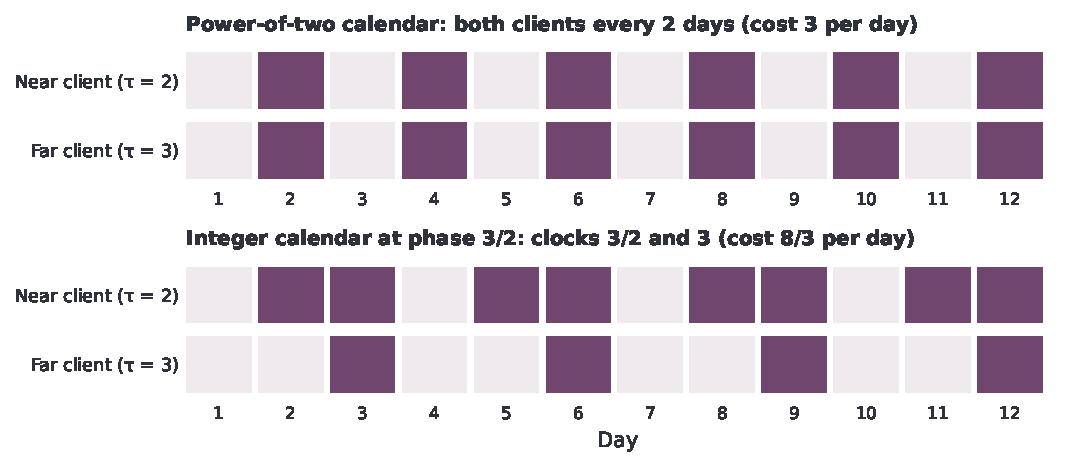
\includegraphics[width=0.8\linewidth,height=\textheight,keepaspectratio,alt={The three-day example. Each row is a client and each column a day; a filled cell is a visit. Top: the power-of-two calendar (cost 3 per day). Bottom: the integer calendar at phase 3/2 (cost 8/3 per day), in which the near client's gaps alternate 2, 1.}]{../figures/calendar_example.pdf}
\caption{The three-day example. Each row is a client and each column a
day; a filled cell is a visit. Top: the power-of-two calendar (cost 3
per day). Bottom: the integer calendar at phase 3/2 (cost 8/3 per day),
in which the near client's gaps alternate 2, 1.}
\end{figure}

\subsection{Independent depot
branches}\label{independent-depot-branches}

Branches at the depot have disjoint edges and disjoint client
constraints, so each branch may choose its own phase. Their daily tours
can be concatenated at the depot, and their average costs add.
Optimising each branch separately therefore never costs more than
imposing one phase on the whole tree, and it preserves (18). In
particular, a star is solved exactly by giving each leaf its own
turnover as its period.

This refinement changes the cycle-length statement: each branch repeats
within its own largest turnover, but the combined cycle may be the least
common multiple of the branch cycles. Its binary description still has
polynomial length. The statement \(P\le\tau_{\max}\) in Theorem 1 refers
to the single-calendar construction. Each branch may also be shifted in
time by its own start offset without changing feasibility or average
cost, which can spread the daily workload.

\section{Synchronisation and stronger tree lower
bounds}\label{synchronisation-and-stronger-tree-lower-bounds}

The frequency bound (16) assumes that every positive-cost edge can be
used at exactly its minimum frequency simultaneously. Nested edges can
prevent this. We first solve the smallest such obstruction exactly.

\subsection{The nested two-edge
problem}\label{the-nested-two-edge-problem}

Let the activation days of a lower edge be contained in those of the
edge above it. Their maximum gaps are integers \(1\le a\le b\), and
their costs per activation are \(u,v\ge0\). Write \(b=ma+r\), where
\(m=\lfloor b/a\rfloor\ge1\) and \(0\le r<a\).

\textbf{Theorem 2 (exact two-edge optimum).} If \(r=0\), the optimum
average is \(u/a+v/b\). If \(r>0\), it is

\[
C_2(a,b;u,v)=
\min\left\{\frac ua+\frac v{ma},\,
\frac{(m+1)u+v}{b}\right\} \tag{19}
\]

\[
=\frac ua+\frac vb+
\min\left\{\frac{a-r}{ab}u,\,
\frac r{mab}v\right\}. \tag{20}
\]

\textbf{Proof.} Partition a cyclic schedule into the gaps, of lengths
\(d\le b\), between consecutive activations of the lower edge. Both
endpoints of a gap also activate the upper edge. Counting the right
endpoint and excluding the left, a gap of length \(d\) contains at least
\(\lceil d/a\rceil\) activations of the upper edge, so its cost is at
least \(u\lceil d/a\rceil+v\). The overall average is therefore at least
a duration-weighted average of

\[
\frac{u\lceil d/a\rceil+v}{d},\qquad d=1,\ldots,b. \tag{21}
\]

(Extra activations of the upper edge only add cost.) For fixed
\(\lceil d/a\rceil\), (21) is nonincreasing in \(d\), so only \(d=ka\)
for \(1\le k\le m\) and \(d=b\) can minimise it. At \(d=ka\), the value
\(u/a+v/(ka)\) is smallest for \(k=m\). This proves that the optimum is
at least (19). Both candidates are achievable. For \(d=ma\), activate
the upper edge every \(a\) days and the lower edge every \(ma\) days.
For \(d=b\), repeat a block of upper-edge gaps \(a,\ldots,a,r\) (with
\(m\) copies of \(a\)) and activate the lower edge at each block
endpoint. Subtracting \(u/a+v/b\) gives (20). If \(r=0\), use the first
construction with lower-edge period \(b\). \(\square\)

The argument also bounds any noncyclic schedule: incomplete end gaps
have length at most \(b\), and their bounded contribution vanishes in
the average. A strictly positive penalty requires \(u,v>0\) and \(r>0\).

For the three-day example, \(a=2\), \(b=3\), \(u=2\) and \(v=4\).
Formula (19) gives \(\min\{3,8/3\}=8/3\), and (20) adds \(1/3\) to the
frequency bound \(7/3\).

\subsection{When the frequency bound is
exact}\label{when-the-frequency-bound-is-exact}

\textbf{Theorem 3 (divisibility criterion).} For a rooted tree with
nonnegative edge costs, the following statements are equivalent:

\begin{enumerate}
\def\labelenumi{\arabic{enumi}.}
\tightlist
\item
  A feasible repeating schedule has average cost \(L_T\).
\item
  The infimum of feasible average costs equals \(L_T\).
\item
  Whenever a positive-cost edge \(e\) lies above a positive-cost edge
  \(g\), \(q_e\) divides \(q_g\).
\end{enumerate}

\textbf{Proof.} Suppose a repeating schedule attains \(L_T\). Every
positive-cost edge must then be used with frequency exactly \(1/q_e\).
Its cyclic gaps are positive integers at most \(q_e\), and their average
equals \(q_e\) only if every gap equals \(q_e\). Its activation days
therefore form a full arithmetic progression with difference \(q_e\).
The lower edge's progression is contained in the upper edge's
progression, so the upper period divides the lower period.

Conversely, assume the divisibility condition. For each client \(i\),
let \(e(i)\) be the deepest positive-cost edge on its path to the depot,
and serve \(i\) on all multiples of \(q_{e(i)}\). If its path has no
positive-cost edge, serve it daily. (A client below a zero-cost edge
uses the nearest positive-cost edge further up, if any.) This is
feasible because \(q_{e(i)}\le\tau_i\). Fix a positive-cost edge \(e\).
Every service of a client below \(e\) falls on a multiple of \(q_e\), by
the divisibility condition. Some client below \(e\) has turnover exactly
\(q_e\); its assigned edge has the same subtree minimum, so that client
is served on every multiple of \(q_e\). Edge \(e\) therefore has
activation frequency exactly \(1/q_e\). The calendar repeats after a
common multiple of the finitely many periods and attains \(L_T\).

Finally, if the divisibility condition fails, apply (20) to an offending
pair of positive-cost edges. It gives a strictly positive additive gap
above their two singleton bounds. Adding the other singleton bounds
rules out even a sequence of schedules whose costs approach \(L_T\).
\(\square\)

The condition concerns positive-cost edges only. Contracting zero-cost
edges is optional, but the clients below them must still count in the
subtree minima. Edges on different branches need not satisfy any
divisibility.

\subsection{Pooling two-edge bounds without counting costs
twice}\label{pooling-two-edge-bounds-without-counting-costs-twice}

Let \(\mathcal P\) contain the pairs \((e,g)\) of positive-cost edges,
\(e\) above \(g\), with \(q_e\nmid q_g\). For \(p=(e,g)\), set
\(a=q_e\), \(b=q_g=ma+r\) and

\[
A_p=\frac{a-r}{ab},\qquad B_p=\frac r{mab}. \tag{22}
\]

Consider the linear programme

\[
Z=\max_{z\ge0}\sum_{p\in\mathcal P}z_p \tag{23}
\]

subject, for each positive-cost edge \(e\), to

\[
\sum_{p=(e,g)}\frac{z_p}{A_p}
+\sum_{p=(h,e)}\frac{z_p}{B_p}\le w_e. \tag{24}
\]

\textbf{Theorem 4 (pooled lower bound).} Every feasible schedule
satisfies

\[
\operatorname{OPT}_T\ge L_T+Z. \tag{25}
\]

\textbf{Proof.} For any feasible \(z\), allocate \(z_p/A_p\) of the
upper edge's weight and \(z_p/B_p\) of the lower edge's weight to pair
\(p\). Constraints (24) leave nonnegative residual edge weights. Apply
Theorem 2 to every allocated pair and the singleton frequency bound to
each residual. The baseline terms sum to \(L_T\), and each pair adds
exactly \(z_p\). No independence between pairs is needed, because this
is an additive split of the costs of a single schedule. Optimising over
\(z\) proves (25). \(\square\)

There are at most \(|E|(|E|-1)/2\) variables and \(|E|\) constraints,
with polynomially encoded rational coefficients. Any feasible rational
vector gives a rigorous lower bound; optimality is not needed. The
supplied implementation uses a numerical solver to suggest a vector,
then reconstructs rational values and scales them if necessary so that
every constraint holds exactly. The reported bound is therefore a valid
rational certificate even if the numerical optimum is imperfect. Neither
(25) nor Theorem 3 claims that pairwise obstructions capture every
higher-order cost of synchronisation.

\textbf{Remark (how far the frequency bound can be from the optimum).}
Theorem 1 shows \(\operatorname{OPT}_T\le L_T/\ln2\) on every tree. The
gap can be substantial. Take a \emph{broom}: a trunk of round-trip
weight \(2M\) from the depot to a hub, and \(M\) leaves of round-trip
weight \(4\) below the hub with turnovers \(M,\ldots,2M-1\). (The
certified instances also place a client of turnover \(M\) at the hub;
this constraint is redundant, because the leaf of turnover \(M\) already
forces the trunk to be used at least that often.) Exactly certified
optima (Section 8.3) give \(\operatorname{OPT}_T/L_T=9/8\), \(90/77\),
\(630/529\) and \(3780/3139\approx1.204\) for \(M=2,3,4,5\). No
algorithm can therefore satisfy a universal bound \(C\le\alpha L_T\)
with \(\alpha<3780/3139\), so an analysis that compares only with
\(L_T\) cannot prove a factor below \(1.204\). The true supremum of
\(\operatorname{OPT}_T/L_T\) lies in \([1.204,1/\ln2]\) and is open.

\subsection{Overlapping service
features}\label{overlapping-service-features}

The exactness criterion extends beyond trees to weighted coverage costs

\[
f(S)=\sum_{A\in\mathcal F}w_A\,\mathbf1\{S\cap A\ne\varnothing\},
\qquad w_A>0,\quad \varnothing\ne A\subseteq N.
\]

A feature \(A\) can represent a shared dispatch, site or handling
charge. Let \(q_A=\min_{i\in A}\tau_i\), and for each client put

\[
\ell_i=\operatorname{lcm}\{q_A:A\in\mathcal F,\ i\in A\},
\]

with the empty least common multiple defined as one. The frequency bound
is \(L_{\mathcal F}=\sum_A w_A/q_A\).

\textbf{Theorem 5 (coverage exactness).} A repeating schedule attains
\(L_{\mathcal F}\) if and only if \(\ell_i\le\tau_i\) for every client
\(i\). When this holds, serving client \(i\) on every multiple of
\(\ell_i\) attains the bound.

\textbf{Proof.} In a schedule attaining the bound, each feature is
active with frequency exactly \(1/q_A\) and has maximum gap \(q_A\), so
its active days form an arithmetic progression with difference \(q_A\).
Every service of client \(i\) lies in the progression of each feature
containing \(i\). The intersection of these progressions is nonempty, so
it is an arithmetic progression with difference \(\ell_i\), and any
subset of it has gaps of at least \(\ell_i\). Feasibility forces
\(\ell_i\le\tau_i\).

Conversely, serve client \(i\) at the multiples of \(\ell_i\); the
assumed inequality makes this feasible. For a feature \(A\), every
service of a client in \(A\) falls on a multiple of \(q_A\). Choose
\(j\in A\) with \(\tau_j=q_A\). Since \(q_A\) divides \(\ell_j\) and
\(\ell_j\le\tau_j=q_A\), we have \(\ell_j=q_A\). Feature \(A\) is
therefore active on every multiple of \(q_A\) and on no other day, which
attains its singleton bound. The finitely many integer periods have a
common multiple. \(\square\)

In this finite integer-gap model, the infimum over arbitrary feasible
schedules is also attained by a repeating schedule. Record each client's
age in \(\{0,\ldots,\tau_i-1\}\); the feasible daily actions form a
finite directed graph on these states. A minimum-mean cycle gives a
repeating feasible schedule, and splitting any long walk into cycles
plus a bounded remainder shows that no smaller limiting mean is
possible. This is an existence argument, not a polynomial-time
algorithm: the graph can have \(\prod_i\tau_i\) states. Consequently, if
the coverage criterion fails, no schedule sequence can approach
\(L_{\mathcal F}\) either.

\section{Limits of short cycles and harmonic
ladders}\label{limits-of-short-cycles-and-harmonic-ladders}

A single common harmonic ladder includes the dyadic ladders of Section 3
and also ladders with other integer ratios. Each client receives a real
period \(p_i\le\tau_i\) from the ladder, and its clock is rounded to
integer days as in (7), possibly with a client-specific offset. Offsets
do not change a client's service density \(\min\{1,1/p_i\}\), and the
proof below uses only densities.

\textbf{Theorem 6 (harmonic-ladder barrier).} For each integer
\(M\ge2\), take a star with \(M\) leaves of unit activation cost and
turnover times

\[
M,M+1,\ldots,2M-1.
\]

Its unrestricted optimum is

\[
\operatorname{OPT}_M=H_{2M-1}-H_{M-1}
=\sum_{q=M}^{2M-1}\frac1q, \tag{26}
\]

where \(H_k\) denotes a harmonic number. The minimum cost over
\emph{all} single harmonic ladders, rounded to integer days, is exactly
\(1\). Consequently the worst-case factor of that class is at least

\[
\frac1{H_{2M-1}-H_{M-1}}\longrightarrow\frac1{\ln2}. \tag{27}
\]

Together with Theorem 1, this shows that \(1/\ln2\) is the best factor
the class can guarantee.

\textbf{Proof.} A star has additive edge costs. Serving each leaf every
\(q\) days attains its individual lower bound \(1/q\), so (26) is exact.

Take any harmonic assignment and let \(a=\max_i p_i\le2M-1\). If
\(a<M\), every effective period \(\max\{1,p_i\}\) is at most
\(\max\{1,a\}<M\), so the total cost is at least \(M/\max\{1,a\}>1\). If
\(a\ge M\), a client with turnover \(q<a\) cannot use the largest
period, and harmonicity forces its period to be at most \(a/2\). Because
\(a\ge M\ge2\), we have \(a/2\ge1\), so its effective period after daily
coalescence is also at most \(a/2\). Every other client has effective
period at most \(a\). Therefore

\[
C\ge\frac{M+\#\{q\in\{M,\ldots,2M-1\}:q<a\}}a. \tag{28}
\]

For integer \(a\) in the turnover range, the numerator equals \(a\); for
noninteger \(a\), it equals \(\lceil a\rceil>a\). Thus \(C\ge1\). Giving
every client period \(M\) achieves cost \(1\), is feasible and is
harmonic. Finally, (26) is a Riemann sum converging to
\(\int_1^2 dx/x=\ln2\). \(\square\)

The same octave family is the classical worst case for single-integer
reduction in pinwheel scheduling, where it yields the asymptotic density
threshold \(\ln2\) (Chan and Chin, 1992, 1993), and it mirrors the
Liu--Layland task sets. Theorem 6 is the cost version, for arbitrary
integer-ratio ladders. It is not an approximation-hardness result for
the underlying problem: the witness stars are solved exactly by
independent clocks. It shows only that replacing powers of two with
another shared ladder cannot give a smaller universal factor.

\subsection{A sharp restriction on the global
cycle}\label{a-sharp-restriction-on-the-global-cycle}

The same stars give a stronger obstruction that assumes neither harmonic
clocks nor nested calendars.

\textbf{Theorem 7 (short-cycle barrier).} On the star of Theorem 6, the
optimum over all feasible \(P\)-periodic schedules with integer
\(P\le\tau_{\max}=2M-1\) is exactly \(1\). Thus no algorithm that always
returns a schedule repeating within \(\tau_{\max}\) days can guarantee a
factor below \(1/\ln2\), even on stars. Theorem 1 attains that factor
under this output restriction.

\textbf{Proof.} In a \(P\)-periodic schedule, a client of turnover \(q\)
needs at least \(\lceil P/q\rceil\) services per cycle. (A schedule
whose minimal period is a divisor of \(P\) is also \(P\)-periodic and is
covered.) For \(P<M\), all \(M\) clients need at least one service,
giving cost at least \(M/P>1\). If \(M\le P\le2M-1\), exactly \(P-M\)
turnovers are below \(P\). Each of those clients needs at least two
services and every other client at least one, so the total is at least
\(M+(P-M)=P\) and the average at least one. The common \(M\)-day
calendar achieves one. Combine with (26)--(27). \(\square\)

The restriction concerns the length of the global cycle, not the size of
the description. A longer cycle can still be described briefly: visiting
star leaf \(q\) every \(q\) days attains the unrestricted optimum,
although the combined cycle can be far longer than \(\tau_{\max}\).
Formally, let \(\operatorname{OPT}_{\mathrm{short}}\) be the minimum
cost over feasible calendars with \(P\le\tau_{\max}\). Theorem 1 gives
\(\operatorname{OPT}_{\mathrm{short}}\le\operatorname{OPT}/\ln2\) for
every submodular instance, and the stars show

\[
\sup_{\text{instances with }\operatorname{OPT}>0}
\frac{\operatorname{OPT}_{\mathrm{short}}}{\operatorname{OPT}}
=\frac1{\ln2}. \tag{29}
\]

The supremum holds both for rooted trees and for general monotone
submodular costs. It is approached from below and is not attained.

\textbf{Corollary 2 (the analysis of the algorithm is tight on trees).}
Add a trunk edge of weight \(\varepsilon>0\) between the depot and the
centre of the star of Theorem 6. The tree then has a single depot
branch, so the independent-branch refinement changes nothing. Every
calendar with \(P\le\tau_{\max}\) still costs at least \(1\) on the leaf
edges, while \(\operatorname{OPT}\le\operatorname{OPT}_M+\varepsilon\).
Letting \(M\to\infty\) and \(\varepsilon\to0\) shows that the worst-case
ratio of the full algorithm of Section 4, branch refinement included, is
exactly \(1/\ln2\).

\begin{figure}
\centering
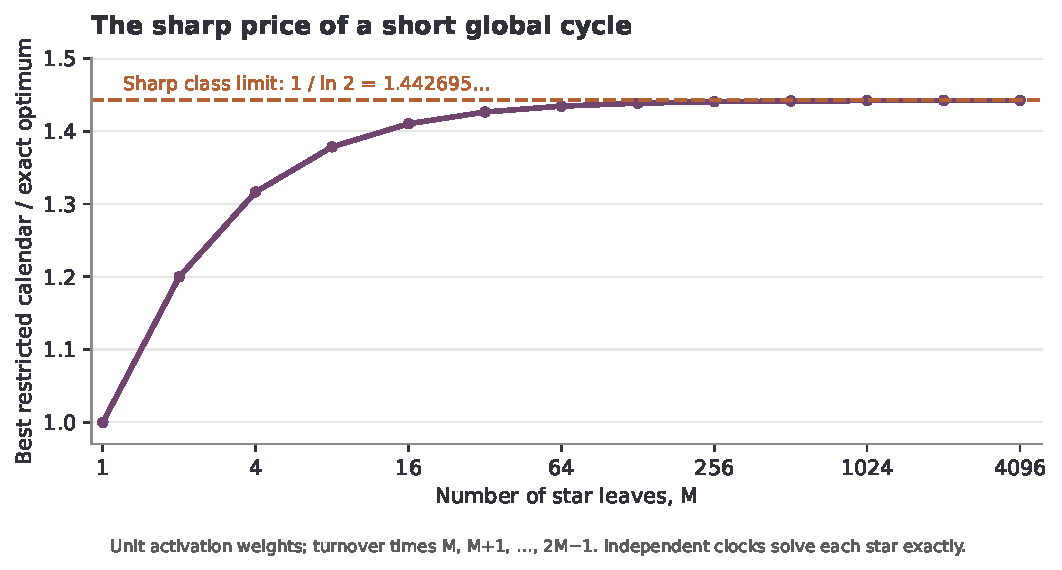
\includegraphics[width=0.95\linewidth,height=\textheight,keepaspectratio,alt={The exact witness ratio approaches the short-cycle and harmonic-ladder limit 1/\textbackslash ln2 from below. Independent clocks attain the unrestricted optimum on each star.}]{../figures/harmonic_class_limit.pdf}
\caption{The exact witness ratio approaches the short-cycle and
harmonic-ladder limit \(1/\ln2\) from below. Independent clocks attain
the unrestricted optimum on each star.}
\end{figure}

\subsection{The full cycle-budget profile of the witness
family}\label{the-full-cycle-budget-profile-of-the-witness-family}

The same stars show how much longer global cycles help. For a prescribed
positive integer cycle \(P\), the exact minimum is

\[
C_M(P)=\frac1P\sum_{q=M}^{2M-1}\left\lceil\frac Pq\right\rceil. \tag{30}
\]

The lower bound comes from counting services. To attain it, place
\(k=\lceil P/q\rceil\) visits to leaf \(q\) as evenly as possible around
the cycle; the largest gap is \(\lceil P/k\rceil\le q\). The leaves have
additive costs and no daily capacity limit, so these placements can
coexist.

\textbf{Theorem 8 (cycle-budget profile).} Define \(H_0=0\) and, for
\(h>0\),

\[
g(h)=\frac1h\int_1^2\left\lceil\frac h x\right\rceil dx.
\]

Writing \(a=\lfloor h/2\rfloor\) and \(b=\lfloor h\rfloor\),

\[
g(h)=H_b-H_a+\frac{1+2a-b}{h}. \tag{31}
\]

This function is continuous and nonincreasing. For every positive
integer budget \(B\),

\[
g(B/M)\le\min_{1\le P\le B}C_M(P)
\le g(B/M)+\frac1M. \tag{32}
\]

In particular, if \(B=\lfloor hM\rfloor\) for fixed \(h>0\), the ratio
of the budget-constrained optimum to the unrestricted star optimum
converges to \(g(h)/\ln2\) as \(M\to\infty\).

\textbf{Proof.} Except at finitely many points,
\(\lceil h/x\rceil=1+\sum_{k\ge1}\mathbf1\{x<h/k\}\). Integrating over
\([1,2]\) gives

\[
\int_1^2\left\lceil\frac h x\right\rceil dx
=1+\sum_{k\ge1}\bigl(\min\{2,h/k\}-1\bigr)_+
=1+2a-b+h(H_b-H_a),
\]

which proves (31). For \(k\ge0\) this reduces to

\[
g(h)=
\begin{cases}
H_{2k}-H_k+1/h,&2k\le h\le2k+1,\ h>0,\\
H_{2k+1}-H_k,&2k+1\le h\le2k+2.
\end{cases}
\]

The pieces meet continuously; they decrease on the first kind of
interval and are constant on the second. At \(h=P/M\), (30) is the left
Riemann sum, divided by \(h\), of the decreasing function
\(x\mapsto\lceil h/x\rceil\) on \([1,2]\) with mesh \(1/M\). The error
of a left sum of a decreasing function lies between zero and (total
decrease)\(/M=(\lceil h\rceil-\lceil h/2\rceil)/M\), so after division
by \(h\) it is at most \((\lceil h\rceil-\lceil h/2\rceil)/(Mh)\).
Finally \(\lceil h\rceil-\lceil h/2\rceil\le h\): the left side is \(0\)
for \(h\le1\), at most \(1<h\) for \(1<h\le2\), and at most
\(h/2+1\le h\) for \(h\ge2\). Hence \(g(P/M)\le C_M(P)\le g(P/M)+1/M\).
Monotonicity of \(g\) gives the lower bound in (32) for every
\(P\le B\), and choosing \(P=B\) gives the upper bound. Continuity and
(26) prove the limit. \(\square\)

For example, \(g=1\) on \([1,2]\), \(g=5/6\) on \([3,4]\) and
\(g=47/60\) on \([5,6]\), giving limiting ratios of about \(1.4427\),
\(1.2022\) and \(1.1301\). These describe this particular family under
the stated budget; they are not improved universal guarantees for
general trees.

\begin{figure}
\centering
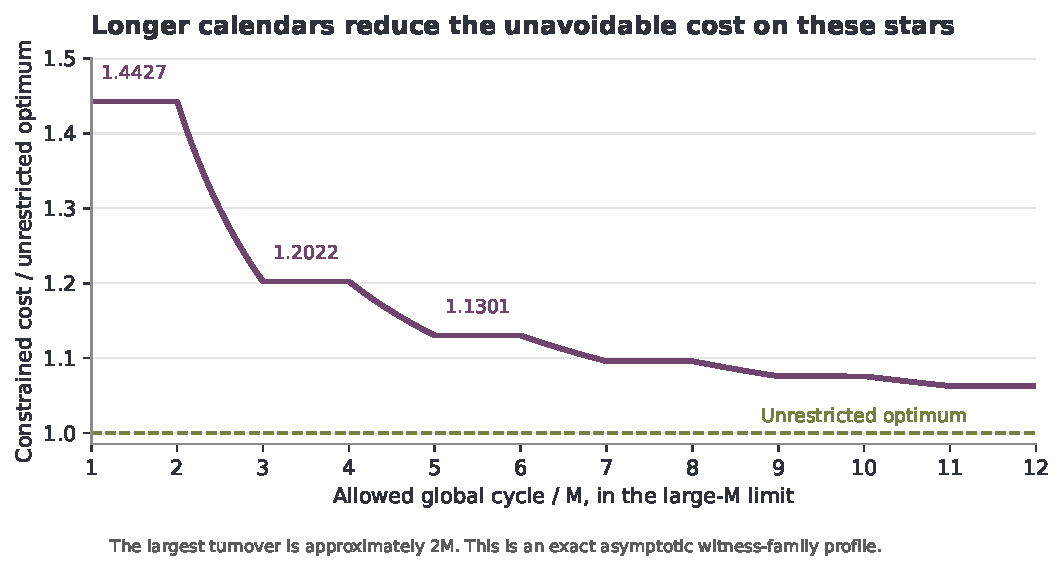
\includegraphics[width=0.95\linewidth,height=\textheight,keepaspectratio,alt={Asymptotic cost of a global cycle budget in the star family. The horizontal variable is the budget divided by M.}]{../figures/cycle_budget_profile.pdf}
\caption{Asymptotic cost of a global cycle budget in the star family.
The horizontal variable is the budget divided by M.}
\end{figure}

\section{The price of constant gaps}\label{the-price-of-constant-gaps}

The calendars of Theorem 1 let a client's gaps alternate. Bosman et
al.'s output keeps every client's gap constant: client \(i\) is visited
every \(p_i\) days, with \(p_i\) an integer power of two. This section
asks how well calendars of that shape can do.

A \textbf{divisor chain} is a sequence \(C=(c_0,c_1,\ldots)\) of
integers with \(c_0=1\) and each \(c_{j+1}\) an integer multiple, at
least twice, of \(c_j\). We consider only chains that, from some top
element \(t\) onwards, continue by doubling (\(t,2t,4t,\ldots\)). For a
turnover \(q\), let \(c_C(q)\) be the largest chain element not
exceeding \(q\). The \textbf{chain calendar} of \(C\) serves client
\(i\) on every multiple of \(c_C(\tau_i)\).

\textbf{Lemma 3 (chain calendars).} A chain calendar is feasible, every
client keeps a constant integer gap \(c_C(\tau_i)\le\tau_i\), and the
calendar repeats within \(\tau_{\max}\) days. Every daily service set is
a prefix \(N_i\), so its average cost is exactly
\(\sum_ia_i/c_C(\tau_i)\). On a tree, each vertex on a day's tour is
also visited with a constant gap, namely \(c_C(q_e)\) for the edge \(e\)
above it, so the calendar is periodic in Bosman et al.'s sense under
either service convention.

\textbf{Proof.} Chain elements divide one another and \(c_C\) is
nondecreasing, so if \(i<j\) then \(c_C(\tau_i)\) divides
\(c_C(\tau_j)\). Every multiple of the larger period is a multiple of
the smaller one, so the service sets are prefixes, and the cost
telescopes as in (9). The largest period used is at most
\(\tau_{\max}\), and every other period divides it. On a tree, edge
\(e\) is active exactly on the multiples of \(c_C(q_e)\), and
\(c_C(q_e)\le q_e\), which is at most the turnover of any client at or
below the vertex it leads to. \(\square\)

For a probability distribution \(\pi\) over finitely many chains, define
the worst-case expected ratio

\[
\rho(\pi)=\sup_{q\ge1}\ \mathbb E_{C\sim\pi}\left[\frac q{c_C(q)}\right]. \tag{33}
\]

By Lemma 3 and linearity, the expected cost of a \(\pi\)-random chain
calendar is
\(\sum_ia_i\,\mathbb E[1/c_C(\tau_i)]\le\rho(\pi)L_f\le\rho(\pi)\operatorname{OPT}\).
Evaluating every chain in the support of \(\pi\) and keeping the
cheapest therefore gives a deterministic constant-gap algorithm with
factor \(\rho(\pi)\), using \(O(n)\) work per chain after sorting.

Computing \(\rho(\pi)\) exactly needs one more observation. Let \(T\) be
the largest top element in the support. For \(q<T\) the supremum is a
finite maximum. For \(q\ge T\), every chain is in its doubling phase,
where \(q/c_C(q)=2^{\{\log_2q-\log_2t_C\}}\).

\textbf{Lemma 4 (tail envelope).} For \(q\ge T\),

\[
\mathbb E_\pi\left[\frac q{c_C(q)}\right]\le\max_{D\in\operatorname{supp}\pi}\ \sum_{C}\pi(C)\,\lambda(t_D/t_C),\qquad
\lambda(x)=\begin{cases}2,&x\text{ an integer power of }2,\\ x/2^{\lfloor\log_2x\rfloor},&\text{otherwise,}\end{cases} \tag{34}
\]

and the bound is approached by integers \(q=t_D2^k-1\) as
\(k\to\infty\).

\textbf{Proof.} Write \(s=\log_2q\) and \(\theta_C=\log_2t_C\). Each
function \(s\mapsto2^{\{s-\theta_C\}}\) is increasing on every interval
between consecutive points of \(\theta_C+\mathbb Z\), and it drops from
(the left limit) \(2\) to \(1\) at those points. The weighted sum is
therefore increasing between consecutive points of
\(\bigcup_C(\theta_C+\mathbb Z)\), and its value anywhere is below its
left limit at the next such point. At a point \(\theta_D+k\), the left
limit of the term for \(C\) is \(\lambda(t_D/t_C)\). Integers just below
\(t_D2^k\) approach that left limit. \(\square\)

\textbf{Theorem 9 (constant-gap harmonic calendars).}

\begin{enumerate}
\def\labelenumi{(\alph{enumi})}
\item
  The two chains \((1,2,4,8,\ldots)\) and \((1,3,6,12,\ldots)\), with
  probabilities \(4/7\) and \(3/7\), give \(\rho=12/7\approx1.714\).
  Adding chains \((1,5,10,\ldots)\) and \((1,4,8,\ldots)\), the
  four-chain mixture with probabilities \(10/29\), \(12/29\), \(5/29\)
  and \(2/29\) on \((1,2,4,\ldots)\), \((1,3,6,\ldots)\),
  \((1,5,10,\ldots)\) and \((1,4,8,\ldots)\) gives
  \(\rho=48/29\approx1.655\). A certified mixture of \(17\) chains with
  top elements at most \(256\) gives \(\rho\le1.60139\). Each is a
  deterministic constant-gap algorithm, for every monotone submodular
  cost and in particular for trees, with that factor and with a cycle of
  at most \(\tau_{\max}\).
\item
  There is a star with \(17\) leaves, with turnovers
  \(2,4,5,7,9,11,15,23,31,47,63,95,127,191,255,383,511\) and explicit
  rational leaf costs, on which every assignment of integer,
  pairwise-dividing periods \(p_i\le\tau_i\) with constant gaps and
  arbitrary offsets costs at least \(1.60010\) times the optimum. The
  same holds after adding a trunk of weight \(\varepsilon\to0\), which
  leaves a single depot branch.
\end{enumerate}

Consequently, the best worst-case factor \(\rho_H\) achievable by
algorithms whose outputs are constant-gap calendars with
pairwise-dividing periods satisfies

\[
1.60010\le\rho_H\le1.60139. \tag{35}
\]

\textbf{Proof.} (a) By Lemma 3, each mixture yields a constant-gap
algorithm with factor \(\rho(\pi)\). The value \(\rho(\pi)\) is the
maximum of finitely many exact rational expressions: the values
\(\mathbb E[q/c_C(q)]\) for \(q<T\), and the left limits (34). The
verifier evaluates them in exact rational arithmetic (Section 8.4). It
obtains exactly \(12/7\) and \(48/29\) for the two- and four-chain
mixtures, and an exact rational below \(1.60139\) for the \(17\)-chain
mixture.

\begin{enumerate}
\def\labelenumi{(\alph{enumi})}
\setcounter{enumi}{1}
\tightlist
\item
  On a star, a leaf with constant gap \(p\) is used on a fraction
  \(1/p\) of the days, whatever its offset, so the cost of a period
  assignment is \(\sum_qw_q/p_q\). Pairwise-dividing integers form a
  divisor chain once \(1\) is added. Assigning each leaf the largest
  chain element not exceeding its turnover is optimal for that chain,
  because the cost decreases as periods grow. With leaf costs
  \(w_q=y_q\,q\) and \(\sum_qy_q=1\), the optimum, attained by
  independent clocks, is \(\sum_qw_q/q=1\). The cost of a chain is
  \(\sum_qy_q\,q/c_C(q)\), which depends only on the chain elements up
  to \(511\). The verifier enumerates all \(15{,}374\) divisor chains
  with elements at most \(511\), checks their number against an
  independent divisor-recursion count, and confirms in exact arithmetic
  that each costs more than \(1.60010\). A trunk of weight
  \(\varepsilon\) adds at most \(\varepsilon\) to the optimum and
  nothing to the leaf costs. \(\square\)
\end{enumerate}

Three points are worth drawing out. First, Theorem 9(a) answers Bosman
et al.'s question even in its narrowest reading: an algorithm whose
output has constant individual gaps, the form they chose, can also beat
two. Second, part (b) shows that forcing such gaps onto one divisibility
ladder costs a definite premium. Variable-gap integer calendars reach
\(1/\ln2\approx1.443\), while constant-gap harmonic calendars cannot do
better than about \(1.600\). The difference comes from integrality: a
real ladder can be shifted continuously, but an integer ladder below its
top element must use divisors. Third, part (b) does not cover constant
gaps that do \emph{not} divide one another, such as the periods \(2\)
and \(3\) in the three-day example. Whether such general constant-gap
policies can reach \(1/\ln2\), or beat it, is open.

The bracket (35) comes from linear programmes over chains with elements
up to \(256\) (upper bound) and \(512\) (lower bound). The proposed
numerical weights are rounded to rationals and then checked exactly.
Smaller caps give \(48/29\) (cap \(8\)) and \(1.6038\) (cap \(64\)) for
the upper bound, and the two bounds approach each other as the caps
grow.

\section{Reproducibility and computational
checks}\label{reproducibility-and-computational-checks}

The mathematical claims above are proved analytically, apart from the
finite certificates for Theorem 9 and the broom remark, which are exact
rational computations. The other finite checks test the implementation,
boundary cases and the link between schedules and cost formulas; they do
not establish the general theorems or historical novelty. All instances
are synthetic. All checkers were written within the same AI-assisted
research session, so ``independent'' below means separately written
code, not independent people.

\subsection{Independent calendar
implementation}\label{independent-calendar-implementation}

A separately written checker does not import the production calendar
code. It enumerates all \(4,680\) ordered turnover tuples of lengths one
to four with every turnover in \(\{1,\ldots,8\}\), tests every candidate
phase and simulates a complete cyclic calendar. It also builds modular,
coverage and binary matroid-rank cost functions.

{\def\LTcaptype{none} % do not increment counter
\begin{longtable}[]{@{}lr@{}}
\toprule\noalign{}
Verified property & Number of checks \\
\midrule\noalign{}
\endhead
\bottomrule\noalign{}
\endlastfoot
Candidate calendars & 11,566 \\
Individual cyclic maximum gaps & 44,838 \\
Modular, coverage and matroid cost instances & 14,040 \\
Exact simulated-cost/formula equalities & 34,698 \\
Rational certifications of the sharpened logarithmic bound & 14,040 \\
Comparisons against an auxiliary phase grid & 14,040 \\
Subday clocks included & 2,718 \\
\end{longtable}
}

The logarithmic inequality is certified with a rational upper bound on
\(\ln2\) from the convergent \(\operatorname{atanh}(1/3)\) series.
Calendar arithmetic uses exact fractions; decimal ratios are for
display. The checker also evaluates the witness stars up to \(M=4096\).

\subsection{Independent two-edge
calculation}\label{independent-two-edge-calculation}

A separate implementation builds the finite age-state graph for two
nested edges. Its state records the time since each edge was last used,
and its actions are no activation, upper edge only, or both. A
stationary-flow linear programme computes the minimum mean-cycle cost.
Across \(532\) combinations of maximum gaps and positive or zero costs,
the numerical optima agree with (19), with largest discrepancy
\(1.78\times10^{-15}\). These are numerical cross-checks; the
closed-form theorem and exact examples carry the claim.

\subsection{Small trees with exactly certified optimal
schedules}\label{small-trees-with-exactly-certified-optimal-schedules}

The comparative benchmark contains \(192\) synthetic instances: \(180\)
fixed-seed cases spread across stars, paths and random trees, and \(12\)
constructed examples. They have two to four clients and turnovers at
most six, and they place a client at every vertex other than the depot
(the theorems also allow Steiner vertices). Each instance is converted
separately into a finite age-state graph whose actions are feasible
daily tours from the depot. A numerical circulation solver suggests an
optimum. A directed cycle then certifies an achievable rational cost,
and integer potential inequalities certify that no cycle has a smaller
mean. All \(192\) optima, and the four broom optima of Section 5.3, have
such exact certificates in the data files.

The state graph starts from all-zero ages, and this loses no periodic
regime. Prepend a visit to every client and then follow any feasible
cycle: the initial ages can only be smaller, which keeps the schedule
feasible, and once each client has been served once (within
\(\tau_{\max}\) days) the ages agree with that regime. For a candidate
mean \(\mu=a/b\), the certificate checks an integer potential \(h\) with
\(h(u)-h(v)\le b\,c(u,v)-a\) on every transition. Summing around any
directed cycle shows that its mean cost is at least \(\mu\), and the
supplied cycle attains \(\mu\). A standard-library verifier, which
imports neither the production code nor a solver, checks all \(48,979\)
transition inequalities, \(1,873\) attaining-cycle steps and \(51\)
rational pair allocations for the \(192\) benchmark trees.

{\def\LTcaptype{none} % do not increment counter
\begin{longtable}[]{@{}
  >{\raggedright\arraybackslash}p{(\linewidth - 6\tabcolsep) * \real{0.2000}}
  >{\raggedleft\arraybackslash}p{(\linewidth - 6\tabcolsep) * \real{0.2667}}
  >{\raggedleft\arraybackslash}p{(\linewidth - 6\tabcolsep) * \real{0.2667}}
  >{\raggedleft\arraybackslash}p{(\linewidth - 6\tabcolsep) * \real{0.2667}}@{}}
\toprule\noalign{}
\begin{minipage}[b]{\linewidth}\raggedright
Measure
\end{minipage} & \begin{minipage}[b]{\linewidth}\raggedleft
Power-of-two (Bosman et al.)
\end{minipage} & \begin{minipage}[b]{\linewidth}\raggedleft
Single-phase calendar (Theorem 1)
\end{minipage} & \begin{minipage}[b]{\linewidth}\raggedleft
Separate depot branches
\end{minipage} \\
\midrule\noalign{}
\endhead
\bottomrule\noalign{}
\endlastfoot
Mean ratio to optimum & 1.170888 & 1.037547 & 1.004514 \\
Median ratio & 1.106203 & 1.000000 & 1.000000 \\
Largest ratio & 1.500000 & 1.250000 & 1.140000 \\
Exact optima attained & 61 & 122 & 179 \\
\end{longtable}
}

The single-phase calendar beats the power-of-two calendar in \(94\)
cases. Separate depot branches improve further through an exact
decomposition, without changing the universal factor. The sample is
small, deliberately stratified and synthetic, so these averages describe
the checks; they do not estimate typical operational savings.

The frequency bound is exact in \(151\) cases, and the rationally
verified pooled-pair bound in \(191\). The one remaining gap has parent
vector \((0,1,1,3)\), edge lengths \((6,7,2,1)\) and client turnovers
\((4,5,5,3)\), where node \(0\) is the depot and each entry describes
the next numbered node. Its edge turnovers are \((3,5,3,3)\), and

\[
L_T=44/5,\qquad L_T+Z=48/5,\qquad
\operatorname{OPT}_T=C_T=10.
\]

So the pooled bound can stay strictly below the optimum even when the
constructed calendar is optimal. All divisibility-criterion predictions
and all executed calendar costs agree with the certificates. The largest
reachable state graph has \(480\) states and \(4,851\) transitions.
These small instances understate the gap between the frequency bound and
the optimum; the brooms of Section 5.3 show larger gaps.

\begin{figure}
\centering
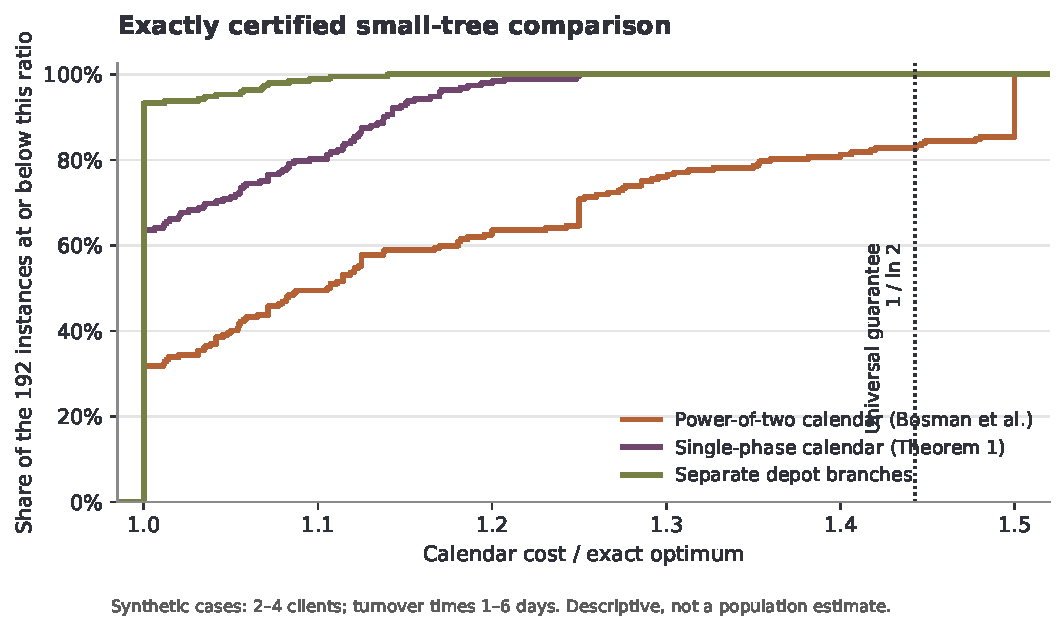
\includegraphics[width=0.95\linewidth,height=\textheight,keepaspectratio,alt={The empirical distribution of cost ratios on the 192 exactly certified synthetic trees. Lower ratios are better. Separate depot branches improve the implementation but do not change the universal factor.}]{../figures/benchmark_ecdf.pdf}
\caption{The empirical distribution of cost ratios on the 192 exactly
certified synthetic trees. Lower ratios are better. Separate depot
branches improve the implementation but do not change the universal
factor.}
\end{figure}

\subsection{Constant-gap certificates}\label{constant-gap-certificates}

A numerical linear programme proposes the chain mixtures and the star
weights of Theorem 9. A standard-library verifier then recomputes every
bound in exact rational arithmetic. For mixtures, it evaluates
\(\mathbb E[q/c_C(q)]\) for every integer \(q\) below the largest top
element and every left limit (34), and it confirms the envelope on
explicit large integers. For the lower bound, it enumerates every
divisor chain with elements at most \(511\) and checks the count against
an independent recursion. It reproduces \(12/7\) and \(48/29\) exactly,
and it certifies \(\rho\le1.6013817\) and \(\rho_H\ge1.6001012\).

\subsection{Coverage and cycle-budget
checks}\label{coverage-and-cycle-budget-checks}

The coverage criterion was tested against \(100\) exactly certified
finite-state optima, \(58\) attaining the bound and \(42\) with strict
gaps, with no disagreement. The coverage audit builds its own model but
reuses cycle and potential routines from the tree benchmark. Complete
certificates for all \(100\) cases come with a separate standard-library
verifier, which checks \(115,378\) integer transition inequalities and
\(549\) attaining-cycle steps. As a small example, take unit-cost
features \(\{1,3\}\) and \(\{2,3\}\). Turnovers \((2,3,6)\) attain the
bound \(5/6\). Changing only the third turnover to \(5\) leaves the
bound unchanged but raises the exact optimum to \(1\), as the
least-common-multiple condition predicts.

The cycle-budget checker enumerates binary cyclic service patterns in
\(110\) small cases to confirm the minimum count \(\lceil P/q\rceil\).
It then checks \(3,464\) exact finite-period cases and \(3,464\)
cycle-budget cases, including the endpoints in (31)--(32).

\subsection{Reproduction and evidence
boundary}\label{reproduction-and-evidence-boundary}

From the bundle root, \texttt{python\ verification/run\_verification.py}
runs the whole sequence. It first verifies the shipped certificates as
released, both normally and under \texttt{python\ -O}. It then
regenerates every computation into a separate replay directory, compares
the regenerated optimum values and counts with the shipped data, and
runs negative controls. In those controls, corrupted certificates (a
wrong optimum, a broken potential inequality, a broken cycle, an altered
coverage record) must be rejected, and they are. No check relies on
\texttt{assert} statements, so all checks remain active under
\texttt{python\ -O}. The production calendar and the verifiers need only
Python's standard library; the numerical searches need NumPy and SciPy.
No proof-assistant formalisation was carried out.

\section{What the results mean, and their
limits}\label{what-the-results-mean-and-their-limits}

\emph{Three kinds of regularity.} A planner may want (i) a short global
cycle, so that the whole network's pattern repeats quickly; (ii)
constant gaps for each client (``your machine is restocked every 9
days''); or (iii) alignment with the working week. The main theorem
delivers (i): its calendar repeats within the longest turnover, and
Theorem 7 shows that \(1/\ln2\) is exactly what (i) costs in the worst
case. It does not deliver (ii). Theorem 9 delivers (i) and (ii) together
at a worst-case factor of about \(1.60\). On the witness stars, the
optimal policy has (ii) but not (i): each client keeps its own constant
gap, and the global pattern repeats only after a very long time. Theorem
8 quantifies how longer global cycles reduce the cost there. A
prescribed weekly cycle \(P=7k\) can be read off (30) for that family.
In plain numbers, a factor of \(1/\ln2\) means at most about 44\% above
the best achievable long-run routing cost, and on the small benchmark
the median calendar was optimal.

\emph{Peak days.} Nested calendars serve every client on the last day of
the cycle, so the busiest day can cost much more than the average. In
the three-day example the daily costs are \(0,2,6\), a peak \(2.25\)
times the average. Fleet size is often set by the peak. Separate depot
branches can be shifted by different start days to spread the load
without changing the average. Controlling the peak, the min--max
objective of Bosman et al., remains open for these calendars.

\emph{When the model fits.} The model assumes deterministic, constant
consumption, so each \(\tau_i\) is fixed; every day is a working day; an
early visit costs only its routing; and the network is a tree, or more
generally the daily cost is submodular. Leaf edges can represent fixed
costs per stop. A distributor of fuel or gas cylinders on a branching
rural network, with contractual maximum gaps and costs per kilometre,
fits well. Urban cash machines with weekend demand peaks do not, unless
\(\tau_i\) is shrunk conservatively to a service-level quantile. The
model has no vehicle capacity, daily working-time limit, holding cost,
lead time or stochastic demand. General road networks need not give
submodular daily costs, so the result does not resolve general-metric
replenishment.

\emph{Implementation.} A day's service set takes \(O(n)\) membership
tests, and the tree tour is then built in linear time. A turnover
written in binary affects the calendar description only logarithmically.
Printing every day of a long cycle is neither necessary nor polynomial
in the input size.

\emph{What remains open.} The complexity of the tree problem; whether
general constant-gap policies can reach \(1/\ln2\); the exact value of
\(\rho_H\); the supremum of \(\operatorname{OPT}_T/L_T\), now known to
lie in \([1.204,1.4427]\); and whether longer structured cycles on trees
with shared trunks can beat \(1/\ln2\) universally.

\emph{Priority.} The rounding, the cost representation, the phase sweep
and the constant have substantial precedent, credited in Section 1.3.
The Hermansen thesis could not be inspected and might contain an
equivalent or stronger result. The appropriate status is a proved
research candidate with bounded novelty evidence.

\section{Data, code and status}\label{data-code-and-status}

Code, certificates, data, figures and logs are archived with this paper
at \url{https://doi.org/10.5281/zenodo.23845965} (concept DOI
10.5281/zenodo.23845964) and at
\url{https://github.com/ipitchford/integer-calendar-replenishment}, tag
\texttt{v1.0.0-candidate}. The release page is
\url{https://evidencepress.org/releases/integer-calendar-replenishment/}.
Text and data are CC0-1.0; code is MIT. This is an unrefereed research
candidate.

\section{Research and verification
statement}\label{research-and-verification-statement}

The construction, proofs, computational checks and literature audit were
developed with AI assistance. Separate AI agents carried out
mathematical challenges, independent implementations and an internal
multi-perspective review, whose findings led to this release: the
constant-gap results, the tightness corollary, the broom remark, the
expanded credit to prior work and hardened verification code. This was
internal checking, not external peer review. No empirical data, author
correspondence, journal acceptance or formal verification is claimed.
The bundled files contain the exact claims, executable checks and search
boundary, so that a specialist can reproduce and assess the work.

\clearpage

\section{References}\label{references}

\subsection{Mathematical and logistics
sources}\label{mathematical-and-logistics-sources}

Anily, S., Glass, C. A., \& Hassin, R. (1998). The scheduling of
maintenance service. \emph{Discrete Applied Mathematics, 82}(1--3),
27--42. \url{https://doi.org/10.1016/S0166-218X(97)00119-4}

Bar-Noy, A., Bhatia, R., Naor, J., \& Schieber, B. (2002). Minimizing
service and operation costs of periodic scheduling. \emph{Mathematics of
Operations Research, 27}(3), 518--544.
\url{https://doi.org/10.1287/moor.27.3.518.314}

Becchetti, L., Marchetti-Spaccamela, A., Vitaletti, A., Korteweg, P.,
Skutella, M., \& Stougie, L. (2009). Latency-constrained aggregation in
sensor networks. \emph{ACM Transactions on Algorithms, 6}(1), 1--20.
\url{https://doi.org/10.1145/1644015.1644028}

Bhat, A., \& Rajkumar, R. (2023). \emph{Assigning optimal integer
harmonic periods to hard real time tasks} {[}Preprint{]}. arXiv.
\url{https://arxiv.org/abs/2302.03724}

Bienkowski, M., Böhm, M., Byrka, J., Chrobak, M., Dürr, C., Folwarczný,
L., Jeż, Ł., Sgall, J., Thang, N. K., \& Veselý, P. (2020). Online
algorithms for multilevel aggregation. \emph{Operations Research,
68}(1), 214--232. \url{https://doi.org/10.1287/opre.2019.1847}

Bienkowski, M., Byrka, J., Chrobak, M., Dobbs, N., Nowicki, T.,
Sviridenko, M., Świrszcz, G., \& Young, N. E. (2015). Approximation
algorithms for the joint replenishment problem with deadlines.
\emph{Journal of Scheduling, 18}(6), 545--560.
\url{https://doi.org/10.1007/s10951-014-0392-y}

Bosman, T. (2019). \emph{Relax, round, reformulate: Near-optimal
algorithms for planning problems in network design and scheduling}
{[}Doctoral thesis, Vrije Universiteit Amsterdam{]}. CWI repository.
\url{https://ir.cwi.nl/pub/29320}

Bosman, T., \& Olver, N. (2020). Improved approximation algorithms for
inventory problems. In \emph{Integer Programming and Combinatorial
Optimization} (Lecture Notes in Computer Science, pp.~91--103).
Springer. \url{https://doi.org/10.1007/978-3-030-45771-6_8}

Bosman, T., van Ee, M., Jiao, Y., Marchetti-Spaccamela, A., Ravi, R., \&
Stougie, L. (2018). Approximation algorithms for replenishment problems
with fixed turnover times. In \emph{LATIN 2018: Theoretical Informatics}
(Lecture Notes in Computer Science, pp.~217--230). Springer.
\url{https://doi.org/10.1007/978-3-319-77404-6_17}

Bosman, T., van Ee, M., Jiao, Y., Marchetti-Spaccamela, A., Ravi, R., \&
Stougie, L. (2022). Approximation algorithms for replenishment problems
with fixed turnover times. \emph{Algorithmica, 84}(9), 2597--2621.
\url{https://doi.org/10.1007/s00453-022-00974-4}

Chan, M. Y., \& Chin, F. Y. L. (1992). General schedulers for the
pinwheel problem based on double-integer reduction. \emph{IEEE
Transactions on Computers, 41}(6), 755--768.
\url{https://doi.org/10.1109/12.144627}

Chan, M. Y., \& Chin, F. (1993). Schedulers for larger classes of
pinwheel instances. \emph{Algorithmica, 9}(5), 425--462.
\url{https://doi.org/10.1007/BF01187034}

Cheung, M., Elmachtoub, A. N., Levi, R., \& Shmoys, D. B. (2016). The
submodular joint replenishment problem. \emph{Mathematical Programming,
158}(1--2), 207--233. \url{https://doi.org/10.1007/s10107-015-0920-3}

Coelho, L. C., Cordeau, J.-F., \& Laporte, G. (2014). Thirty years of
inventory routing. \emph{Transportation Science, 48}(1), 1--19.
\url{https://doi.org/10.1287/trsc.2013.0472}

Díaz-Ramírez, A., Mejía-Alvarez, P., \& Leyva-del-Foyo, L. E. (2013).
Comprehensive comparison of schedulability tests for uniprocessor
rate-monotonic scheduling. \emph{Journal of Applied Research and
Technology, 11}(3), 408--436.
\url{https://doi.org/10.1016/S1665-6423(13)71551-7}

Federgruen, A., \& Zheng, Y.-S. (1992). The joint replenishment problem
with general joint cost structures. \emph{Operations Research, 40}(2),
384--403. \url{https://doi.org/10.1287/opre.40.2.384}

Federgruen, A., \& Zheng, Y.-S. (1993). Optimal power-of-two
replenishment strategies in capacitated general production/distribution
networks. \emph{Management Science, 39}(6), 710--727.
\url{https://doi.org/10.1287/mnsc.39.6.710}

Fujiwara, H., Miyagi, K., \& Ouchi, K. (2026). Pinwheel scheduling with
real periods. \emph{Discrete Mathematics \& Theoretical Computer
Science, 28}(4). \url{https://doi.org/10.46298/dmtcs.17657} {[}Abstract
inspected.{]}

Gąsieniec, L., Jurdziński, T., Klasing, R., Levcopoulos, C., Lingas, A.,
Min, J., \& Radzik, T. (2024). Perpetual maintenance of machines with
different urgency requirements. \emph{Journal of Computer and System
Sciences, 139}, 103476. \url{https://doi.org/10.1016/j.jcss.2023.103476}

Han, C.-C., \& Lin, K.-J. (1992). Scheduling distance-constrained
real-time tasks. In \emph{Proceedings Real-Time Systems Symposium}
(pp.~300--308). IEEE. \url{https://doi.org/10.1109/REAL.1992.242649}
{[}Full text not inspected.{]}

Han, C.-C., Lin, K.-J., \& Hou, C.-J. (1996). Distance-constrained
scheduling and its applications to real-time systems. \emph{IEEE
Transactions on Computers, 45}(7), 814--826.
\url{https://doi.org/10.1109/12.508320} {[}Full text not inspected.{]}

Holte, R., Mok, A., Rosier, L., Tulchinsky, I., \& Varvel, D. (1989).
The pinwheel: A real-time scheduling problem. In \emph{Proceedings of
the Twenty-Second Annual Hawaii International Conference on System
Sciences} (Vol. 2, pp.~693--702). IEEE.
\url{https://doi.org/10.1109/hicss.1989.48075}

Kawamura, A. (2024). Proof of the density threshold conjecture for
pinwheel scheduling. In \emph{Proceedings of the 56th Annual ACM
Symposium on Theory of Computing} (pp.~1816--1819). ACM.
\url{https://doi.org/10.1145/3618260.3649757}

Liu, C. L., \& Layland, J. W. (1973). Scheduling algorithms for
multiprogramming in a hard-real-time environment. \emph{Journal of the
ACM, 20}(1), 46--61. \url{https://doi.org/10.1145/321738.321743}

Mohaqeqi, M., Nasri, M., Xu, Y., Cervin, A., \& Årzén, K.-E. (2018).
Optimal harmonic period assignment: Complexity results and approximation
algorithms. \emph{Real-Time Systems, 54}(4), 830--860.
\url{https://doi.org/10.1007/s11241-018-9304-0}

Nagarajan, V., \& Shi, C. (2016). Approximation algorithms for inventory
problems with submodular or routing costs. \emph{Mathematical
Programming, 160}(1--2), 225--244.
\url{https://doi.org/10.1007/s10107-016-0981-y}

Nonner, T., \& Souza, A. (2009). Approximating the joint replenishment
problem with deadlines. \emph{Discrete Mathematics, Algorithms and
Applications, 1}(2), 153--173.
\url{https://doi.org/10.1142/S1793830909000130}

Roundy, R. (1985). 98\%-effective integer-ratio lot-sizing for
one-warehouse multi-retailer systems. \emph{Management Science, 31}(11),
1416--1430. \url{https://doi.org/10.1287/mnsc.31.11.1416}

Roundy, R. (1989). Rounding off to powers of two in continuous
relaxations of capacitated lot sizing problems. \emph{Management
Science, 35}(12), 1433--1442.
\url{https://doi.org/10.1287/mnsc.35.12.1433} {[}Publisher abstract
inspected.{]}

Segev, D. (2026). \emph{Resource-constrained joint replenishment via
power-of-\(m^{1/k}\) policies} {[}Preprint{]}. arXiv.
\url{https://arxiv.org/abs/2603.18720}

Teo, C.-P., \& Bertsimas, D. (2001). Multistage lot sizing problems via
randomized rounding. \emph{Operations Research, 49}(4), 599--608.
\url{https://doi.org/10.1287/opre.49.4.599.11222}

van Ee, M. (2021). A 12/7-approximation algorithm for the discrete
Bamboo Garden Trimming problem. \emph{Operations Research Letters,
49}(5), 645--649. \url{https://doi.org/10.1016/j.orl.2021.07.001}

Zhang, Y., \& Kulkarni, V. (2018). Automated teller machine
replenishment policies with submodular costs. \emph{Manufacturing \&
Service Operations Management, 20}(3), 517--530.
\url{https://doi.org/10.1287/msom.2017.0656} {[}Publisher abstract
inspected.{]}

\subsection{Priority-boundary record}\label{priority-boundary-record}

Bille, P. (n.d.). \emph{Students and supervision: MSc., BSc., and B.Eng.
theses}. Technical University of Denmark. Retrieved 31 October 2026,
from \url{https://people.compute.dtu.dk/~phbi/people.html} {[}Lists
Hermansen's Spring 2025 MSc thesis; the thesis itself could not be
obtained.{]}

\end{document}
